\chapter[Annexes]{Annexes}
\thispagestyle{firstpage}

\minitoc
\newpage

\section{Article 3}\label{article3}
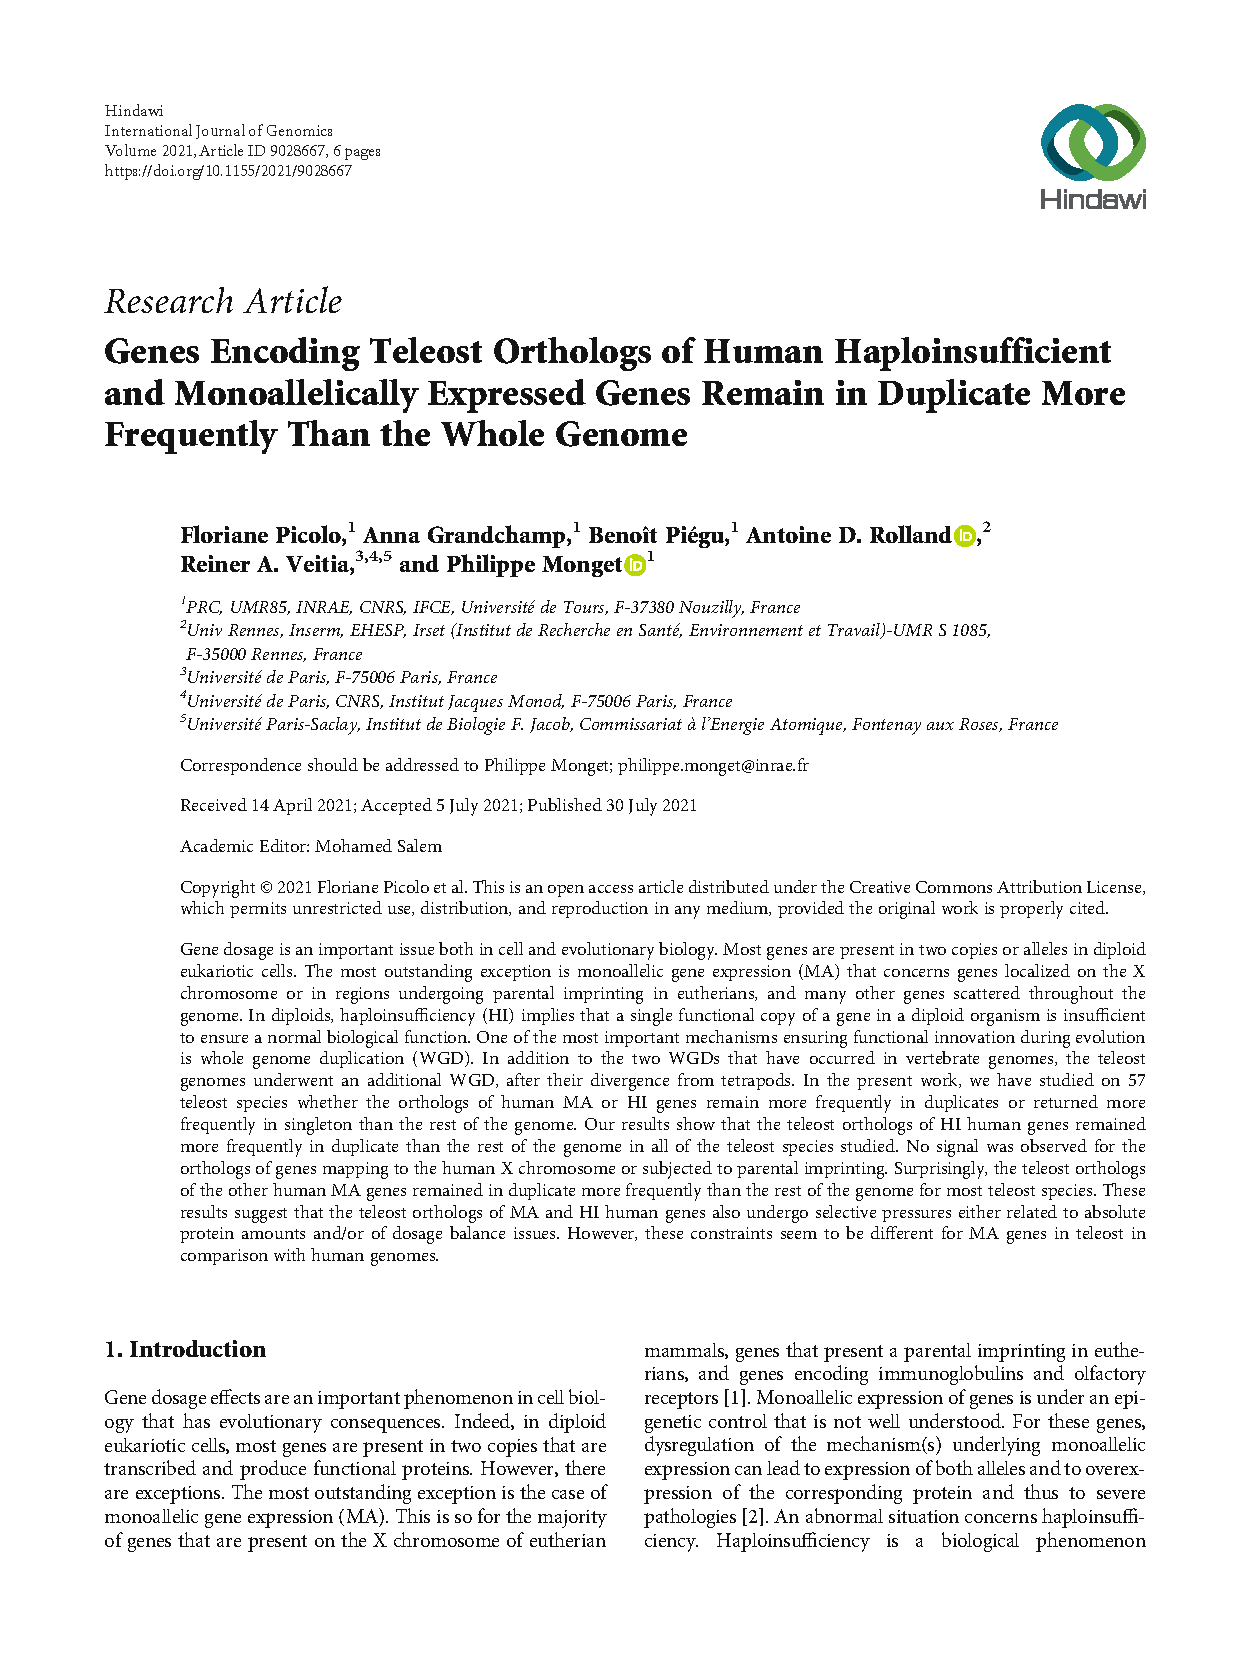
\includepdf[scale=0.85,pages=1-6,pagecommand={\thispagestyle{plain}}]{figures/articles/pico-2023.pdf}

\section{Article 1 - Suppl. Data 1}
\textbf{Suppl. Data 1 - Distribution of deltas of node of birth of genes encoding proteins involved in all the pathways, according to the node of birth of each gene}\\
Legend: Deltas are calculated via clade of birth rank for the A gene - clade of birth rank for the B gene for the interaction A $\rightarrow$ B. For example, if gene A was born at the blue clade (clade 1), and the clade of birth of B is 11, the A $\rightarrow$ B delta is -10. Moreover, in this case, it is a backward relationship, because A was born before B.
\par The pathways are in the following order:
p53, AGE-RAGE, Adipocytokine, Estrogen, Glucagon, GnRH, Insulin, Ovarian steroidogenesis, Oxytocin, PPAR, Prolactin, Relaxin, Thyroid hormone, B cell receptor, C-type lectin receptor, Chemokine, FC epsilon RI, IL-17, NOD-like receptor, RIG-I-like receptor, T cell receptor, Toll-like receptor, Neurotrophin, AMPK, Apelin, Calcium, cAMP, cGMP-PKG, ErbB, FoxO, Hedgehog, HIF-1, Hippo, JAK-STAT, MAPK, mTOR, NF-Kappa B, Notch, Phospholipase D, PI3K-Akt, Rap1, Ras, Sphingolipid, TGF-Beta, TNF, VEGF, Wnt.

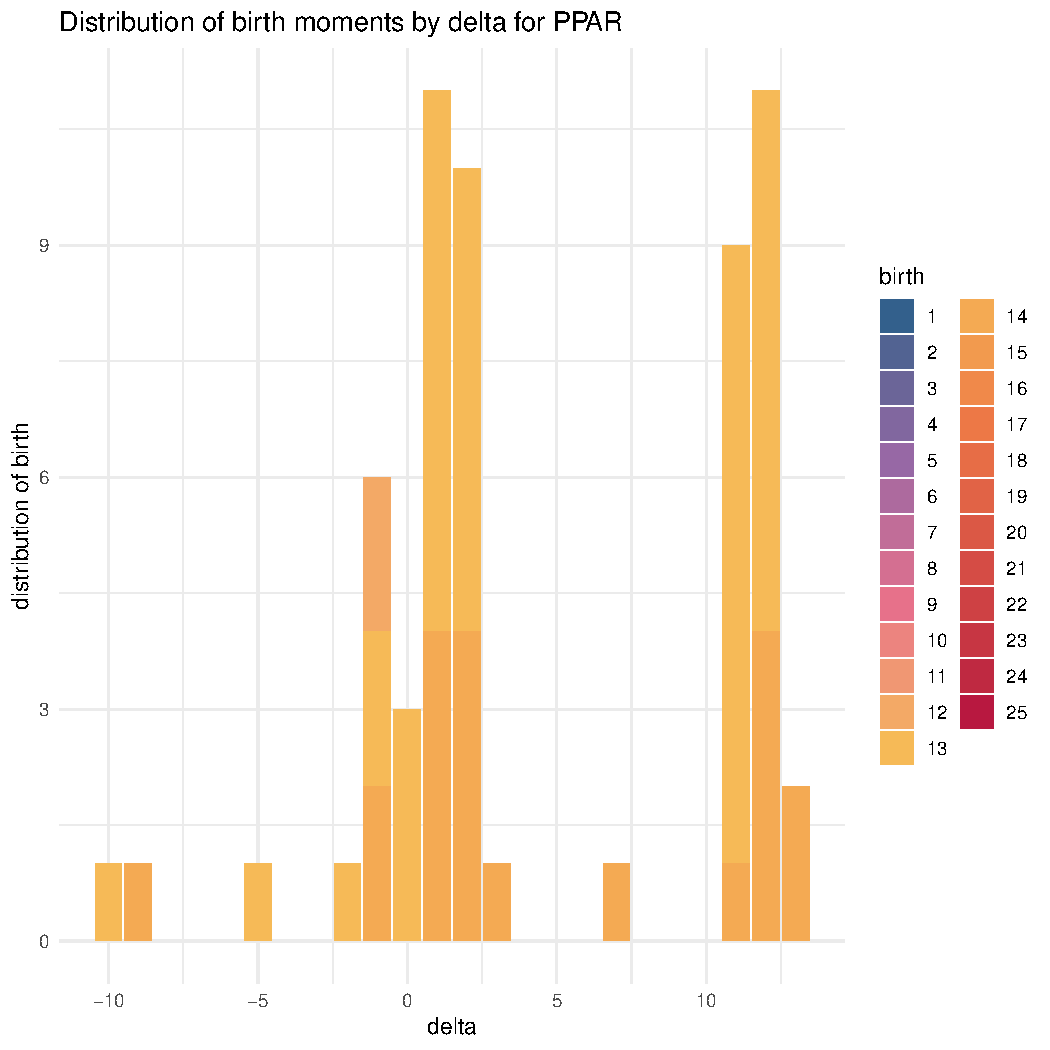
\includepdf[scale=0.85,pages=1-47, nup=1x2, pagecommand={\thispagestyle{plain}}]{figures/suppldata/suppldata1.pdf}

\section{Article 1 - Suppl. Data 2}
\textbf{Suppl. Data 2 - Distribution of genes by position/rank in the pathway and node of birth}\\
Legend: Each graph represents one of the 47 pathways. Abscissa: the different proteins involved in the pathway; ordinate: position/rank of the protein within the pathway. Each protein is colored depending on the node of birth of its corresponding gene. Proteins are represented by a dot, are characterized by their position(s) they occupy within the pathway. The size of the dots is proportional to the number of times they are in these positions.
\par The pathways are in the following order:
p53, AGE-RAGE, Adipocytokine, Estrogen, Glucagon, GnRH, Insulin, Ovarian steroidogenesis, Oxytocin, PPAR, Prolactin, Relaxin, Thyroid hormone, B cell receptor, C-type lectin receptor, Chemokine, FC epsilon RI, IL-17, NOD-like receptor, RIG-I-like receptor, T cell receptor, Toll-like receptor, Neurotrophin, AMPK, Apelin, Calcium, cAMP, cGMP-PKG, ErbB, FoxO, Hedgehog, HIF-1, Hippo, JAK-STAT, MAPK, mTOR, NF-Kappa B, Notch, Phospholipase D, PI3K-Akt, Rap1, Ras, Sphingolipid, TGF-Beta, TNF, VEGF, Wnt.

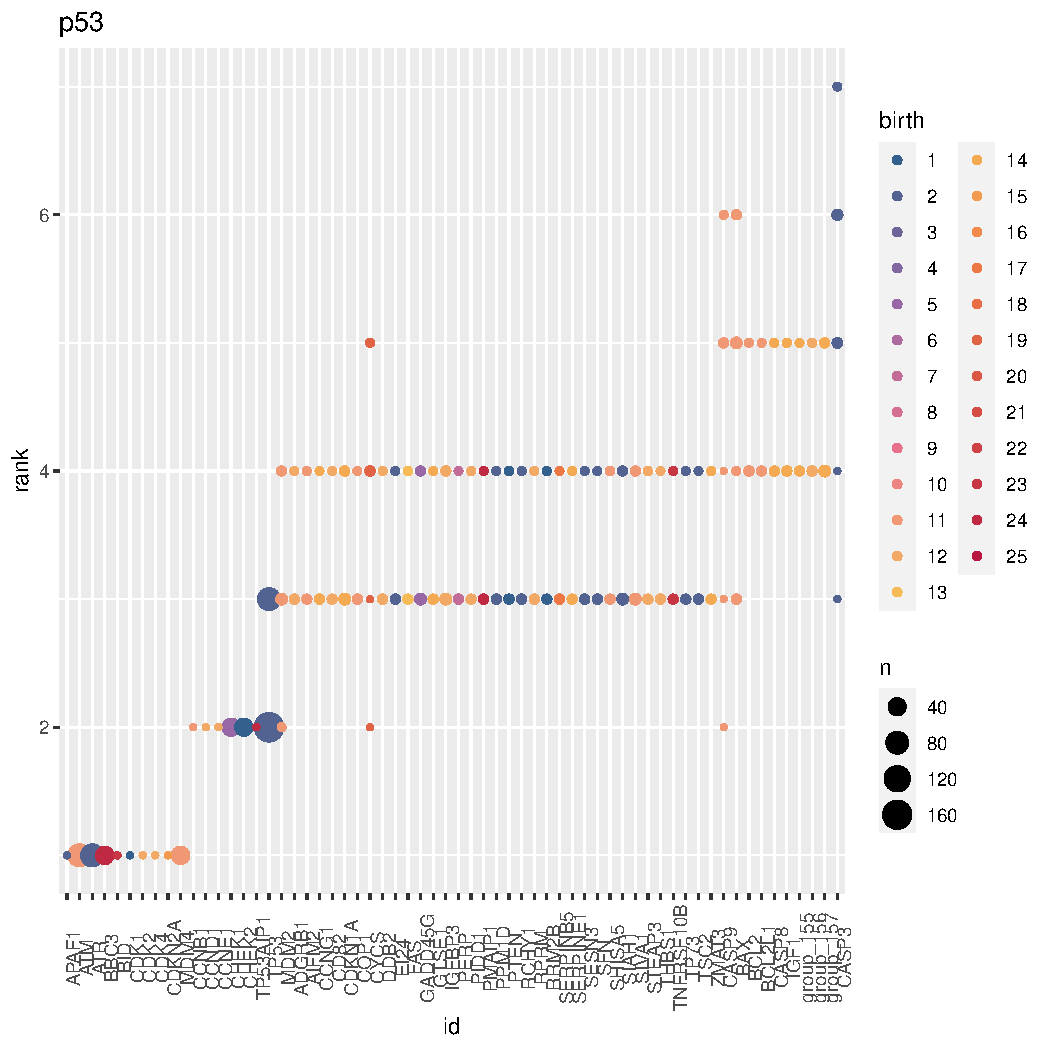
\includepdf[scale=0.85,pages=1-47, nup=1x2, pagecommand={\thispagestyle{plain}}]{figures/suppldata/suppldata2.pdf}

\section{Article 1 - Suppl. Data 3}
\textbf{Suppl. Data 3 - Colored KEGG pathways depending on the node of birth of each protein}\\
Legend: Each color represents a clade. The white rectangles correspond to the genes for which we have not been able to determine the node of birth due to lack of information about the gene. The KEGG legend is available here: \href{https://www.genome.jp/kegg/document/help_pathway.html}{https://www.genome.jp/kegg/document/help}
